% Explore the strategy of varying dialect by observing openvpn
% (1) tightening constraint on edge can remove unwanted or vulnerable component
% (2) preserving constraint on edge can also cause the change to outfacing interface
% (3) relaxing constraint is not a good idea because (1) introducing non-deterministic (2) enlarge attack surface
% (4) Add new states
% (5) Remove states through message removal
% (6) Add State though introducing new messages

\begin{figure*}[t]
\centering
\subfloat[Original Dialect.]{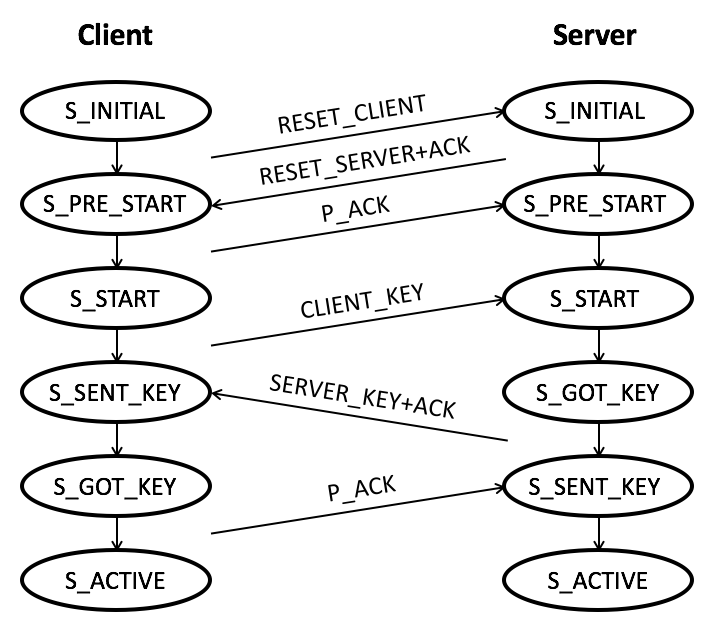
\includegraphics[width=0.33\linewidth]{figure/openvpn_protocol}\label{fig:original_dialect}} 
\subfloat[Dialect with state removal.]{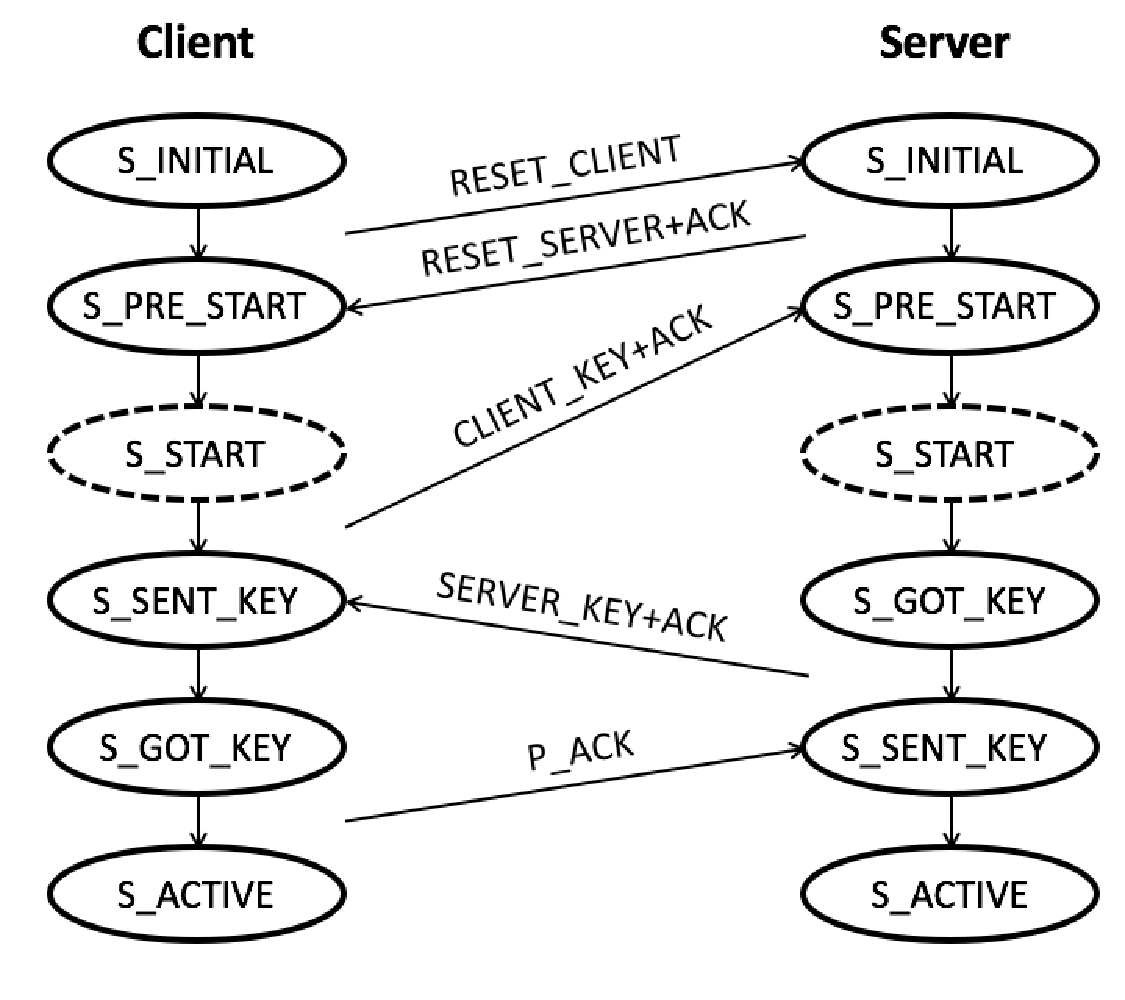
\includegraphics[width=0.33\linewidth]{figure/mutation4}\label{fig:detleted_dialect}}
\subfloat[Dialect with state addition.]{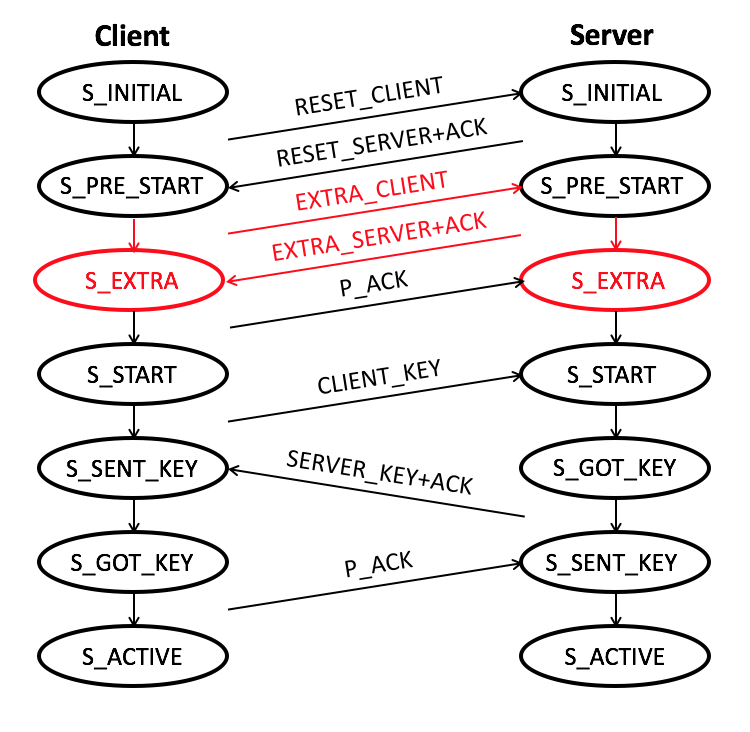
\includegraphics[width=0.33\linewidth]{figure/mutation3}\label{fig:added_dialect}} 
\vspace{-0.1in}
\caption{The protocol dialects implemented in \texttt{OpenVPN} responsible for establishing a private communication tunnel.} 
\label{fig:dialect} 
\end{figure*} 


\section{Generating Various Dialects}
\label{sec:dialect}

With finite state machines extracted, we now discuss how we plan to customize
protocol implementation to generate various dialects. In the following, we discuss the challenge of dialect generation followed by our proposed techniques.


\subsection{Challenges}
\label{sec:task2:challenges}

Dialect generation needs to take as input a protocol implementation, and generate
various dialects. To achieve
this, we have to address two major challenges below.


\noindent{\textbf{Consistency.}} A communication protocol typically involves
more than one parties exchanging messages between each other. Typically,
implementations pertaining to such protocols might be separated into different
code bases and even involved in multiple parties. When performing protocol dialect generation, we must modify protocol implementation across different code bases. Given the complicated control flow and data dependency in source code, the second challenge of dialect generation is to develop a generic approach to handle the consistency of code variation.

\noindent{\textbf{Validity.}} 
To generate a new dialect, there are many possible approaches. However, many of them may not guarantee the reliability (or validity) of a dialect newly generated (\eg, generating a new dialect for \texttt{TCP} communication by eliminating the three-way handshake). As a result, the first challenge of dialect generation is to identify a set of effective strategies that can generate new protocol dialects but not introduce incorrectness. 

\subsection{The Proposed Techniques}

We propose a series of technical approaches to tackle the aforementioned challenges. As is mentioned above, dialect gneration requires code modification which could potentially introduce code inconsisitent variation. As a result, we first discuss how we plan to address this issue using a static analysis approach. Following this proposed technique, we then discuss three possible approaches to generate a new dialect without jeopardizing protocol validity. It should be noticed that our effort for dialect generation is not limited to these three approaches. Throughout this research project, we will also explore other strategies and techniques for dialect generation.

\subsubsection{Research Task 4: Linking Code Bases across Multiple Parties}

To address the code inconsistency variation issue, we must have a mechanism to link code bases across multiple parties. In this project, we intend to utilize a static analysis technique. To be specific, we will first identify the finite state machines that involve communication dialects. Since a communication dialect involves message exchanging, we intend to achieve this by examining state machines tied to function calls responsible for message sending and receiving. Second, we will pair state machines tied to the same dialect. To accomplish this, we plan to examine the data structure tied to function calls. Here, our hypothesis is that, if sending and receiving function calls are all tied to the same data structure, the corresponding state machines are involved to the same dialect. In this project, we will validate this hypothesis and -- if needed -- adjust this technique based on protocol implementations. 

After identifying and pairing state machines, we will then recover the sequence of the messages exchanged between the paired state machines. To do this, we plan to  perform value set analysis on the code base corresponding to each of the state machines. Similar to the technique proposed for refining a state machine in Section~\ref{}, we will conduct this analysis against the outgoing messages prior to its attachment to message sending, and then match that value set with transition conditions of the state machine present on the other side. To illustrate this approach, we take \texttt{OpenVPN} for example. By performing a value set analysis at the site where a client state machine sends a request message, we obtain a set of values for the message which perfectly match transition condition \Code{!(&ks->plaintext_write_buf->len) && !session->opt->server && packet.opcode == P_CONTROL_HARD_RESET_CLIENT_V2} present on the edge of a server state machine. 

With protocol dialect restored, it is not difficult to notice that one could easily pinpoint the messages exchanged between each other. Since the dialect is recovered through a static analysis approach, he or she can easily track down the code of interest as well as those relevant to that code fragment. To illustrate this, we take for example one of the dialects implemented in \texttt{OpenVPN} (see Figure~\ref{fig:original_dialect}). By tracing back message \texttt{P\_ACK} to its sender, we can pinpoint the call to that function responsible for sending that message. Taking the call as a sink, we could easily identify the code fragments relevant to message \texttt{P\_ACK} by performing a backward taint analysis.

\subsubsection{Research Task 5: Generating Dialects with Message Partition}

\subsubsection{Research Task 6: Generating Dialects with Message Merging}

\subsubsection{Research Task 7: Generating Dialects with Message Elimination}

We will also explore dialect generation through messag elimination. To achieve this, one possible solution is to tighten the transition condition present on a finite state machine. Take for example \texttt{OpenSSL}, a state machine of which is illustrated in Figure~\ref{}. By removing condition XXX, we could tighten the condition pertaining to the transition from state AAA to BBB. Since this condition removal needs to be reflected to the change of constraints in control flows, we further remove the code fragment dependent upon this cut-off condition. 

Figure~\ref{} illustrates one of the code fragments we trimmed. It indicates the heartbeat component vulnerable to the heartbleed bug~\citep{}. As such, we observe this transition condition tightening not only generates a new dialect which does not involves the heartbeat messages exchanged between a client and a server, but also safeguards \texttt{OpenSSL} against overflow vulnerabilities. Since the heartbeat component is optional for \texttt{OpenSSL}, the dialect newly generated is still valid. In this project, we will further examine this condition tightening scheme for generating new dialects, and explore in what condition this approach can always give us valid dialects. 
